\documentclass[a4paper]{scrartcl}
\usepackage[utf8]{inputenc}
\usepackage[english]{babel}
\usepackage{graphicx}
\usepackage{lastpage}
\usepackage{pgf}
\usepackage{wrapfig}
\usepackage{fancyvrb}
\usepackage{fancyhdr}
\usepackage{listings}
\pagestyle{fancy}
\usepackage{libertine}
\renewcommand*\familydefault{\sfdefault}  %% Only if the base font of the document is to be sans serif
\usepackage[T1]{fontenc}
\usepackage{courier}
\usepackage[parfill]{parskip}

\graphicspath{ {./images/} }

% Create header and footer
\headheight 27pt
\pagestyle{fancyplain}
\lhead{\footnotesize{Internet Applications, ID1354}}
\chead{\footnotesize{Assignment 2: JavaScript}}
\rhead{}
\lfoot{}
\cfoot{\thepage\ (\pageref{LastPage})}
\rfoot{}

% Create title page
\title{Assignment 2: JavaScript}
\subtitle{Internet Applications, ID1354}
\author{Emil Tullstedt [emiltu@kth.se]}
\date{2014-09-24}

\lstset{
	basicstyle=\footnotesize\ttfamily, 
	numbers=left,
	breaklines=true,
	frame=l,
	keywordstyle=\bfseries\color{blue!40!black},
    stringstyle=\color{red},
    commentstyle=\color{green},
    identifierstyle=\color{black},
    showstringspaces=false
}

\begin{document}

\maketitle

\section{Introduction}

The second assignment for ID1354 is about adding JavaScript functionality to a static web site. The task was to develop the following on the website developed for the first assignment:

\begin{itemize}
\item Create a JavaScript-powered drop-down menu
\item Develop a volatile comment field
\item Make the comments editable and delete-able
\item Add two pages containing static information
\end{itemize}

\section{Method}

\subsection{JavaScript Best Practices}

There are very few programming languages that doesn't need sensible code standards which can be controlled against using a linter. Idiomatic JavaScript is especially hard, as the programming language by default doesn't enforce either it's end-of-line character (the interpreter has to make a guess at where one line of code ends and another one begins) or variable declaration. As the language further isn't safe and has side-effects (this is a property of most imperative languages). JavaScript also has a tendency to silently die, and as the language is written to be non-blocking - might run certain functions ahead of plausible time.

Because of the \textit{flexibility} that JavaScript inherits from this design choice, the language is very prone to software bugs. This has caused several off-spring versions of JavaScript to be developed, but as the language's most important factor is the portability, neither of these versions has ever gained the same momentum as the language itself.

The JSLint tool available to check for JavaScript best-practices at \texttt{jslint.com} is rather strict because of all this. To make the check more suitable for the needs of this assignment, the following comment is inserted at the top of the JavaScript documents that are run through the lint:

\texttt{/*jslint browser: true, vars: true, white: true, indent: 4, maxlen: 80 */}

This silences "bad" placement of variables (i.e. multiple declarations within a single block [there are sensible reasons why you wouldn't want this, but neither are applicable for our case]), "bad" whitespace usage (libraries shouldn't silence this, but whitespace isn't important in JavaScript and can be safely ignored) and assumes the client is a browser. We further suggest an indentation level of 4 spaces (which, as the whitespace error is ignored, is quite unnecessary) and a maximum length of a single line in the document of 80 characters.

You also need to inform JSLint about the global variables, where the JQuery '\$'-variable is the most notable.

Furthermore, because of the issues that the design choices of JavaScript implicates, there is a syntax that allows developer to ask the browser to crash earlier when parsing what looks like invalid JavaScript. This is done by putting \texttt{"use strict";} at the top of either a JavaScript document or a function. The JSLint.com website complains about the use of the "use strict"; in top of the document and proposes you to put it at the top of the functions\footnote{You can do this by enclosing the entire document in an anonymous function - but for this purpose, that just makes the code uglier.} instead, but that is acceptable for non-reusable libraries.

\subsection{•}

\section{Result}
\label{sec:results}

\begin{figure}[!h]
  \begin{center}
    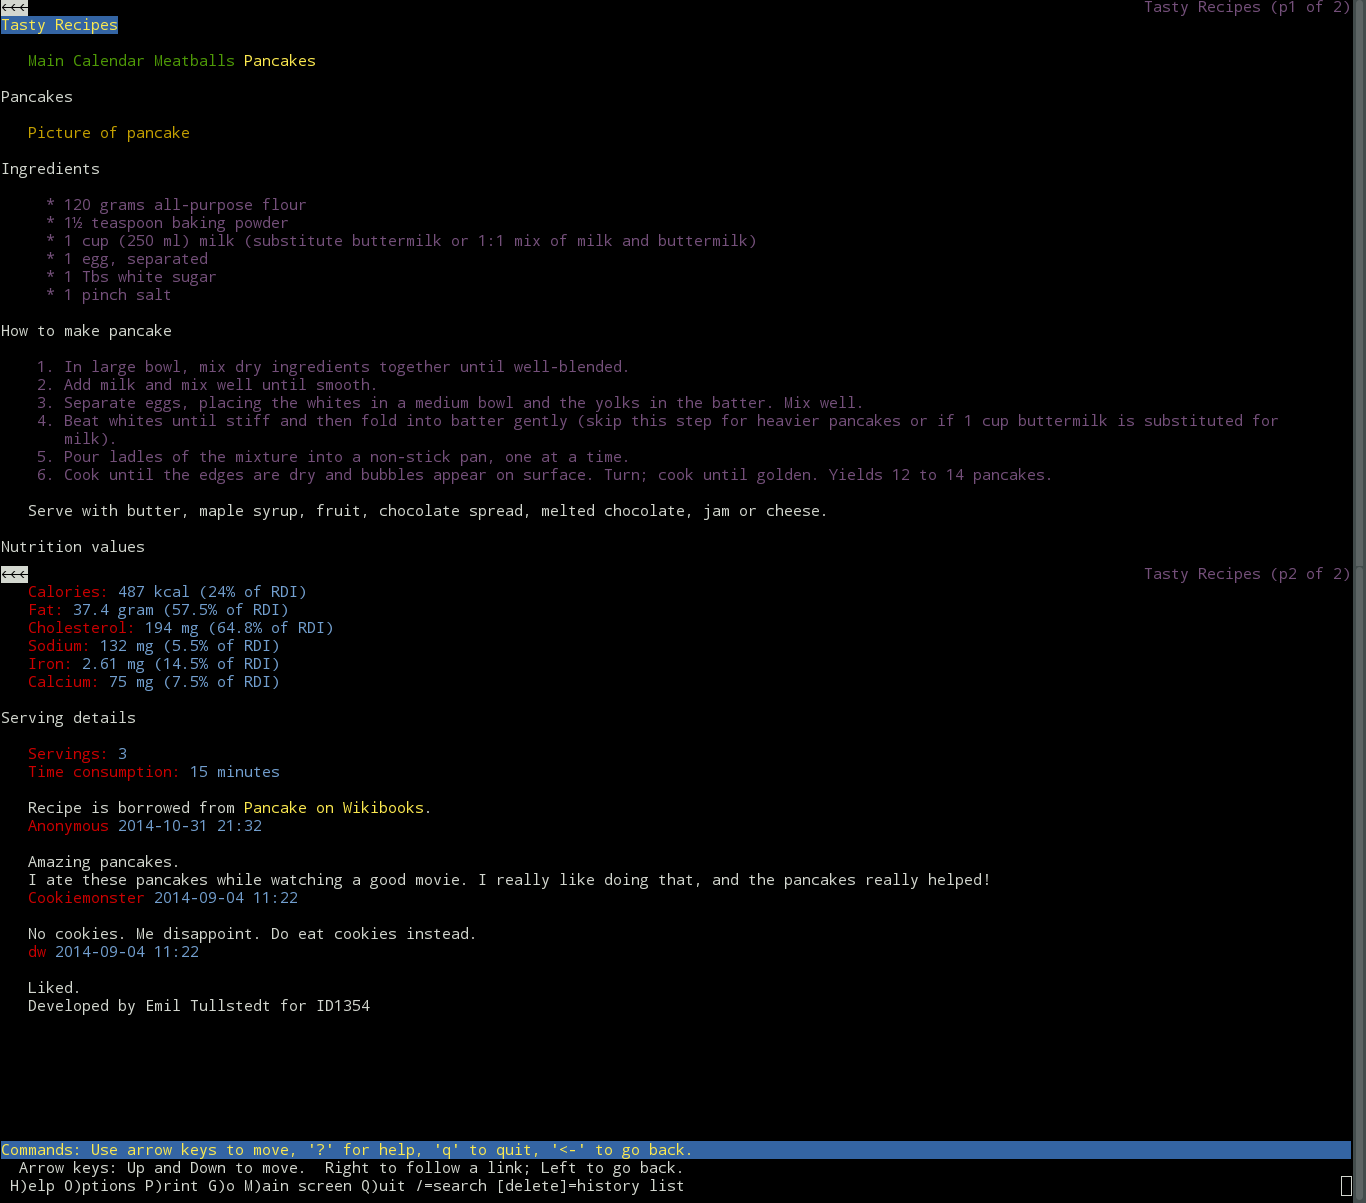
\includegraphics[scale=0.3]{pancakelynxboth.png}
    \caption{The recipe page in a text based browser}
    \label{fig:pancakelynx}
  \end{center}
\end{figure}
\section{Discussion}

\subsection{Basic Requirements}
\begin{itemize}
\item \textbf{Dropdown menu} - See subsection \ref{subsec:dropdown} for details.
\item \textbf{About us and contact us} -
\item \textbf{JSLint} -
\item \textbf{Using JQuery syntax} - 
\end{itemize}

\begin{figure}[!h]
  \begin{center}
    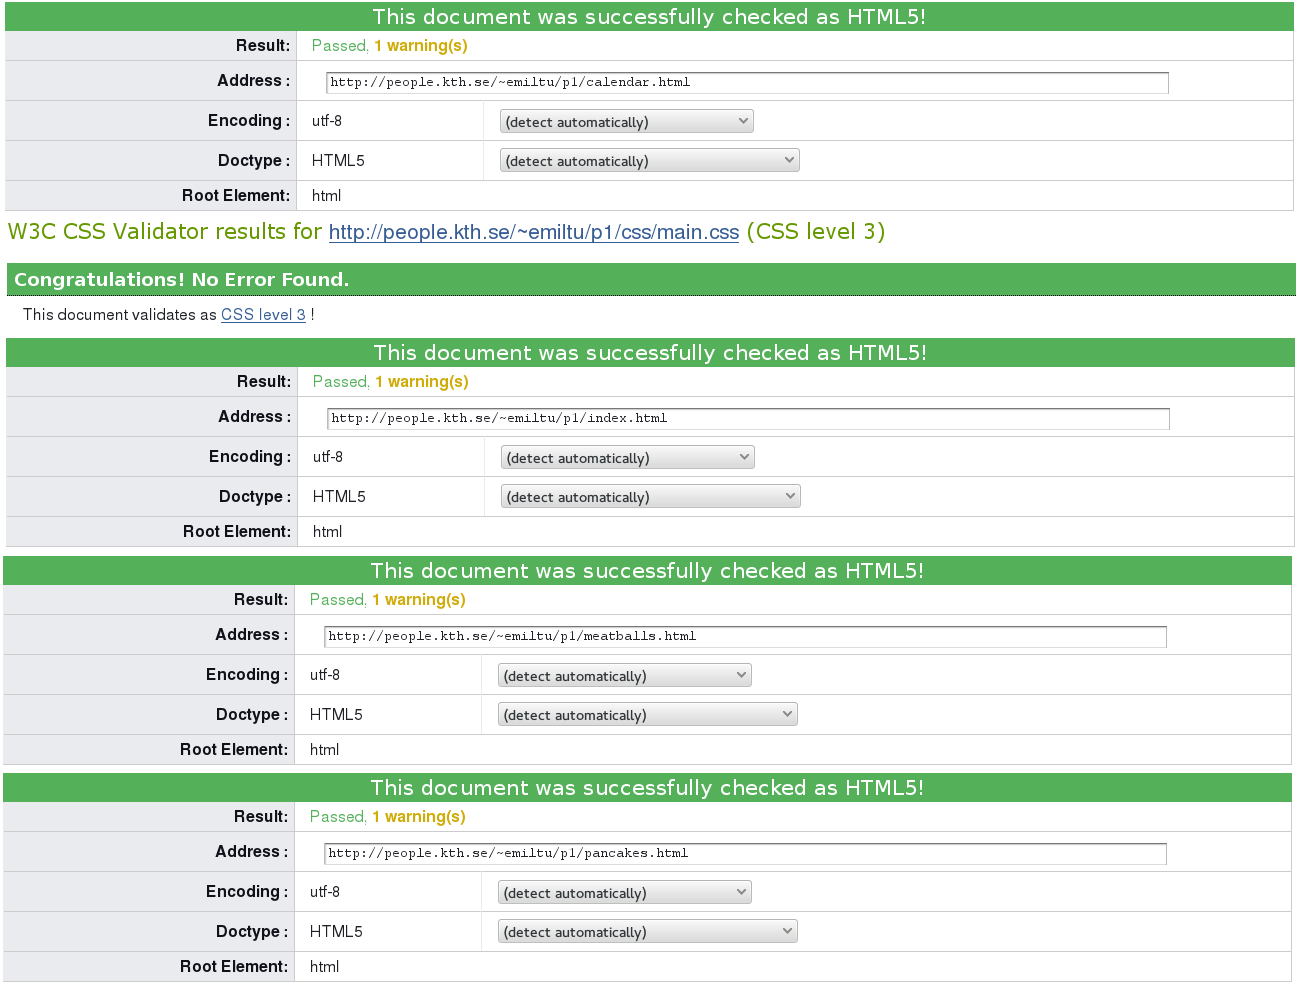
\includegraphics[scale=0.3]{valid.png}
    \caption{Validation results for the different parts of the site}
    \label{fig:valid}
  \end{center}
\end{figure}

\subsection{Adaptiveness}

\begin{figure}[!h]
  \begin{center}
    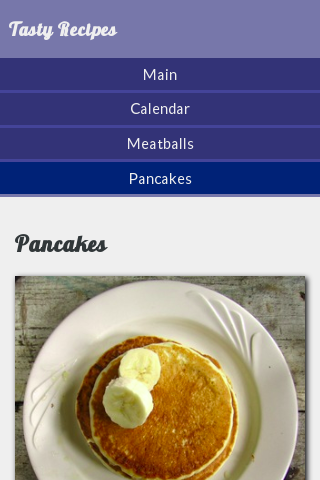
\includegraphics[scale=0.3]{pancakelow1.png}
    \caption{How the menu adapts for lower resolutions}
    \label{fig:menu-adapt}
  \end{center}
\end{figure}

The site is built to feel responsive and work under any browser. By using the built-in Firefox "responsive web development" toolkit this was able to be tested for every change of the page. With the utilization of media queries, the site makes sense on all kinds of different sized screens.

\subsection{Cross-Browser Compatibility}

The site was developed with using "safe" standards in mind, which means that the website \textit{should} work under any modern browser. This was further tested using Microsoft's screenshot service to take screenshots in all different kinds of browsers\footnote{This can be done by the reader by pointing the tool at http://modern.ie/screenshots to the website at http://people.kth.se/$\sim$emiltu/p1}.

\subsection{Web Server Information}
\label{subsec:httpd}

Setting up a web server on Fedora is a matter of \texttt{yum install httpd} and \texttt{systemctl start httpd}. This server can then be extended to accommodate server side page generation, such as PHP or WSGI for Python, which is yet to be done.

\begin{lstlisting}
unary Projects/id1354 $ yum info httpd                                                                                                       
Loaded plugins: langpacks

Installed Packages
Name        : httpd
Arch        : x86_64
Version     : 2.4.10
Release     : 1.fc20
Size        : 3.8 M
Repo        : installed
Summary     : Apache HTTP Server
URL         : http://httpd.apache.org/
License     : ASL 2.0
Description : The Apache HTTP Server is a powerful, efficient, and extensible
            : web server.
\end{lstlisting}

\end{document}
